\documentclass{mprop}
\usepackage{graphicx}

% alternative font if you prefer \usepackage{times}

% for alternative page numbering use the following package and see documentation
% for commands \usepackage{fancyheadings}


% other potentially useful packages \uspackage{amssymb,amsmath}
\usepackage{url}
%\usepackage{fancyvrb} \usepackage[final]{pdfpages}

\begin{document}

%%%%%%%%%%%%%%%%%%%%%%%%%%%%%%%%%%%%%%%%%%%%%%%%%%%%%%%%%%%%%%%%%%%
\title{Is Technical Debt Real?}
\author{Ovidiu Popoviciu}
\date{18th December 2017}
\maketitle
%%%%%%%%%%%%%%%%%%%%%%%%%%%%%%%%%%%%%%%%%%%%%%%%%%%%%%%%%%%%%%%%%%%

%%%%%%%%%%%%%%%%%%%%%%%%%%%%%%%%%%%%%%%%%%%%%%%%%%%%%%%%%%%%%%%%%%%
\tableofcontents
\newpage
%%%%%%%%%%%%%%%%%%%%%%%%%%%%%%%%%%%%%%%%%%%%%%%%%%%%%%%%%%%%%%%%%%%

%%%%%%%%%%%%%%%%%%%%%%%%%%%%%%%%%%%%%%%%%%%%%%%%%%%%%%%%%%%%%%%%%%%
\section{Introduction}\label{intro}

\begin{itemize}
	\item What is technical debt?
	\item What are its applications?
	\item Why is it important?
\end{itemize}

Technical debt - definition \\
What impact does TD have on development?\\ 
How much work effort is wasted on new features on a codebase impacted with
technical debt?\\
Why is it difficult to define such a measure? \\
If such a measurement is known, how could it be managed? \\
What are the advantages of quantifying technical debt interest in the form work
effort? \\

Problem statement: Has the student analysed the problem, stated it clearly, and
justified its importance?

%%%%%%%%%%%%%%%%%%%%%%%%%%%%%%%%%%%%%%%%%%%%%%%%%%%%%%%%%%%%%%%%%%%
\section{Background Survey}

\subsection{Study Design}

\begin{itemize}
	\item Technical debt definition
	\item Types of TD - focus on code debt
	\item Measurement of principal and interest
	\item Measurement of work effort and team productivity
	\item Management of TD
\end{itemize}

\subsection{Definition, Perspectives and Types}

% Ward Cunningham - WyCash Portfolio Management System TODO: expand the
% definition from the paper.
Technical debt is a metaphor termed by Ward Cunningham, in his famous report on
the WyCash Portfolio Management System in 1993 \cite{Cunningham1993}. In the
report, Cunningham mentioned that "\textit{shipping first time code is like
going into debt.}" and that as the system evolves new features would become more
and more difficult to implement. This phenomenon was due to feature-rich
projects being shipped to customers early but poorly written with little or no
consideration to quality and to future work.

\begin{figure}
	\centering
	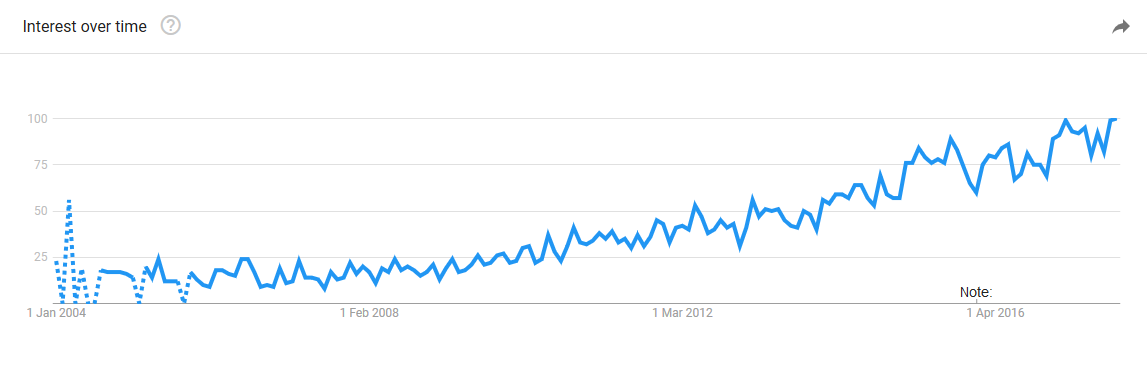
\includegraphics[width=\linewidth]{visualisations/TD_trend.png}
	\caption{Technical Debt Trend from 2004 to Present}
	\label{fig:td-trend}
\end{figure}

% MTD 2010
The metaphor was ignored for a long time, until the late 2000s, when more and
more studies started to explore the phenomenon and possible management
processes. A figure of the popularity of Technical Debt from 2004 to present can
be seen in Figure \ref{fig:td-trend}, information provided by Google Trends
\cite{GoogleTrends}. Thus, the first workshop on managing technical debt took
place in 2010, where an initial research agenda was proposed for the future of
software engineering field. Since then, workshops have been held every year,
which consisted seminars, presentations and brainstorming sessions on aspects
such as definition \cite{Kruchten2012} \cite{Theodoropoulos2011}
\cite{Schmid2013}, identification \cite{Ernst2012}, measurement
\cite{Letouzey2012} \cite{Curtis2012} \cite{Nugroho2011} \cite{Zazworka2011}
\cite{Fontana2012} \cite{Bohnet2011}, management \cite{Guo2011}
\cite{Zazworka2011Prioritise} \cite{Seaman2012} to industry case studies
\cite{Lim2012} \cite{Morgenthaler2012} \cite{Codabux2013} \cite{Holvitie2014}
\cite{Klinger2011}.

% from metaphor to theory and practice TODO: add citation to industry case
% studies
The definition of technical debt relies heavily on the perspective of the viewer
and her responsibility within the socio-technical environment. Developers view
technical debt as a list of software quality issues and correlate it with lack
of time to implement features "\textit{properly}" \cite{Codabux2013}. Product
managers and stakeholders view at it as a strategy, a way to defer quality work
for fast work in order to satisfy certain business requirements, such as Time to
Market (TTM). In practice, these two perspectives are widely different, with
developers prioritising "invisible" code perfection whilst management focusing
on rapid development of "visible", selling point features. Kurchten et al.
\cite{Kruchten2012} defined technical debt as technological gaps between
development teams and management, where a gap is the evolution of a context
specific to a decision taken in the past. These gaps might have been decisions
that seemed correct when the decision was taken however, with the passing of
time, the initial decision incurred debt within the project. For example, there
is no tool that predicts what frameworks and languages will exist in the future
or how to implement features by considering future unknown requirements. As a
consequence, the authors state that technical debt is not the collection of code
quality violations within the results of static code analyzers but, a phenomenon
which is heavily reliant on present and future project evolution.


% from a stakeholder's perspective
However, most strategic decisions on the future evolution of the project come
from management. Unfortunately, stakeholders might not have knowledge of the
metaphor of technical debt, its current measurement and whether it impacts costs
of development. Their main focus of increasing business value through the
addition of visual features, rather than looking for investment in the quality
of the software being produced. As a result, new features are prioritised and
pressured on being delivered as early and as quickly as possible. These types of
issues affect the \textbf{extrinsic quality} of software and are "visible". For
example, an extrinsic quality characteristic is usability. Deferring user
experience work and ignoring user interface bugs might force users of the system
to find "ways around" certain tasks. The result is negative impact in user
productivity and the general usefulness of the product. Extrinsic
characteristics are important to the business as they are considered "sell
points" of the product. On the other hand, \textbf{intrinsic quality}
characteristics of software are the low-level issues such as code smells,
best-practices violations that might slow down development of new features
unless refactoring processes are applied. Theodoropoulos et al.
\cite{Theodoropoulos2011} considered that intrinsic and extrinsic software
quality characteristics are interdependent and deferring quality maitainence in
one area may affect other areas of quality. For example, improper data
validation in the business logic layer of the system, may impact downstream
components, such as user interface, and produce bugs within the system.


% on the limits of td metaphor TODO: define principal and interest
Although the use of finance terms may simplify technical characteristics of
software quality in the dialogue between development teams and stakeholders, the
analogy breaks down as studied by Schimd et al. \cite{Schmid2013}. In their
study, the authors had identified shortcomings in the financial metaphor
established by Ward Cunningham \cite{Cunningham1993} and found points where it
breaks down. In the financial domain, debt is a well known arrangement between
two parties where one party borrowes a fixed amount of money from the other
party \cite{debt-investopedia}. The most well known types of debt are loans,
where the terms of the arrangement dictate that the amount of money borrowed
must be paid back in full after a fixed period of time, along with fixed
interest payments paid annually.

Schmid et al. \cite{Schmid2013} has identified three major points where the
analogy breaks down:
\begin{itemize}
	\item \textit{Unit of measurement}. In finance there is a clear unit of
	      monetary measurement through the use of international currencies. In
	      contrast, technical debt does have a standard unit of measurement
	      defined. There are many tools (TODO: add citation of paper tools
	      here) that provide a single, quantified and aggregated measure of
	      the amount of time it takes for software quality issues to be
	      resolved. Additionally, very few of these tools quantify the
	      consequences of neglecting refactoring and the improvement in
	      quality characteristics. The issue of measurement puts a dent into
	      the shared vocabulary between development and stakeholders as
	      mentioned by a number of software practioners from industry case
	      studies (TODO: add industry case study citation here).
	\item \textit{Fixed time period}. On the one hand, debt arrangements have
	      a fixed \textit{maturity date}, where the debt must be paid back. On
	      the other hand, software quality issues do not a have a time limit
	      and may be kept in the product until they are resolved. Fixing these
	      items relate to paying back the "loan" taken on their creation. Such
	      issues may never be paid back if not needed to, resulting in an
	      increased cost-value ratio.
	\item \textit{Fixed interest}. A loan arrangement additionally consists of
	      fixed interest payments measured as a percetange of the loan value,
	      paid on an annual or bi-annual basis. The interest compensates for
	      the risk taken by the lender and encourages the loanee to pay back
	      quickly as possible in order to avoid paying back too much interest.
	      In reality, there is no such thing as fixed interest dependant on a
	      single factor in technical debt. Interest is difficult to quantify
	      as a matter of principal, and the amount of interest paid after a
	      period of time depends on future work.
\end{itemize}
Under these circumstances, what is considered "good structure" or "clean code"
is also heavily influenced to future development since future decisions
influence cost impact. As a consequence, no system is \textit{debt free} and
thus fixing every code violation would be an act of gold plating. Additionally,
what is the value of paying back this debt if the product is competitive and the
customers are happy \cite{Lim2012}?

% martin fowler - td quadrants
In Martin Fowler's famous article \cite{TDMartin}, he described this type of
future debt as \textbf{inadeverted-prudent} debt. Over time, a project that was
"clean" may find that after a period of time that the initial approach taken
might not have been the best. He considered that developers learn on the job to
perfect their craft as time passes. The four quadrants refer to the types of
technical debt that one might encounter in a software project given the approach
taken by the development team. It was one of the four quandrants he defined, as
shown in Figure \ref{fig:td-quandrants}.

\begin{figure}
	\centering
	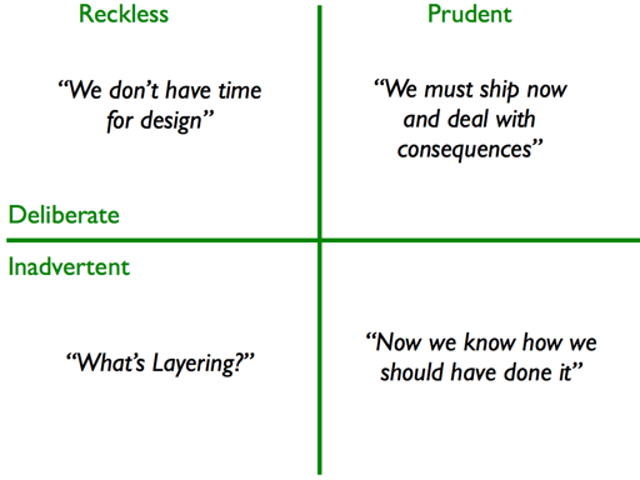
\includegraphics[width=0.5\linewidth]{visualisations/TD_quadrants.png}
	\caption{Martin Fowler's Technical Debt Quadrants}
	\label{fig:td-quandrants}
\end{figure}


% unhedged call option
An alternative metaphor of technical debt \cite{UnhedgedCallOption}, described
bad code using finance terms in a similar fashion, but through a different
financial intrument called a call option.
\textit{An option is a financial derivative that represents a contract sold by
one party (the option writer) to another party (the option holder). The contract
offers the buyer the right, but not the obligation, to buy (call) or sell (put)
a security or other financial asset at an agreed-upon price (the strike price)
during a certain period of time or on a specific date (exercise date).}
\cite{option-investopedia}. A call option gives the right to buy while a put
option gives the option holder the right to sell. In software engineering, if a
feature is hacked up quickly using bad code and never touched again, then the
project had reaped the rewards. The option "was not called". However, if a new
feature were required that would be influenced by the quick and dirty work
implemented earlier, then the requirement would be more expensive to fulfill. In
this case, the option "has been called".


% conclusion
Defining software quality issues as a financial metaphor helps bridge vocabulary
shortcomings between developers and stakeholders. It helps management understand
current software development risks and encourages ways for managing these risks
as they are created. TODO: make sure to write down the exact definition As
Cunningham \cite{Cunningham1993} had written, technical debt may be used as a
strategy in order to meet business expectations however, if not repaid promptly
it could bring entire corporations to a standstill.

% types of TD
Initially, technical debt has solely focused on the internal quality issues of
systems developed. Such issues could be code smells, code violations and
duplicate or complex code. However, multiple types of debt have been
"discovered" spanning the entire socio-technical environment.
% TODO: maybe add a description for all types of debt but only focus on code
% debt
A mapping study, conducted by Li et al. \cite{Li2015}, have analysed 94 papers,
overall dating 1992-2013, and have found 10 types of technical debt being
studied: requirements debt, architectural debt, design debt, code debt, test
debt, build debt, documentation debt, infrastructure debt, versioning debt and
defect debt. The most prominent type of debt studied was code debt, followed by test,
architectural, design and documentation debt.

% architecture debt is the worst - industrial case study
However, in an industrial case study \cite{Codabux2013}, developers considered that
architectural debt is the most difficult to adress, due to complexity and change
impact on project. Major architectural decisions are not taken in a vaccuum and
thus requires group meetings with other developers, software architects and
product managers. The time to reach a consensus on how to approach such changes
improve the cost of managing architectural debt.

% technical debt is "technical"
A few of the authors have considered that the metaphor of technical debt should
only apply to the low-level, internal quality characteristics such as code,
test, architectural debt rather than process gaps such as inadequate quality
assurance \cite{Theodoropoulos2011} \cite{Nugroho2011}. Thus the word
"technical". However, process gaps may negatively affect projects and incurr
technical debt as a result.

%%%%%%%%%%%%%%%%%%%%%%%%%%%%%%%%%%%%%%%%%%%%%%%%%%%%%%%%%%%%%%%%%%%
\subsection{Identification and Measurement}

% What are the causes of code TD?

Technical debt may impede future development and delivery of new features is not
managed appropriately \cite{Cunningham1993}. Cunningham's statement was
validated by a number of authors trying to identify its causes by looking at the
most "notorious" code smells \cite{Fowler1999} and their impact on software projects.

% add software quality impact of code smells here
% - Investigating the Impact of Design Debt on Software Quality
% - Investigating the impact of Code Smells Debt on Quality Code Evaluation
% - Assessing Code Smell Interest Probability
% - An exploratory study on the impact of Code Smells on Software Change-Proneness


% How to quantify code smell impact?



% sqale method for measuring technical debt
The first method the authors looked at was the SQALE method \cite{Letouzey2012}.
The goal was to propose a standardized, language-agnostic framework for
assessing the quality of source code by deriving measures for code
characteristics and calculating an overall measure of technical debt. The
framework proposed consisted of four concepts:
\begin{itemize}
	\item Quality Model - defines internal properties of code through a
	structured three-layer hierarchy (characteristic, sub-characteristic and
	requirement). For example, a characteristic is maintainability,
	sub-characteristic is readability and the requirement is no commented
	code. The hierarchy is defined as all requirements could be converted into
	actionable steps. Each requirement defines a remediation index (cost to
	repair code violations) defined in time, work or capital units.
	\item Analysis Model - measurement of the distance between the current
	state of the application and the \"optimized\" quality target.
	\item Indices - these are the values that represent the costs of paying
	back debt. 
	\item Indicators - provide a visual representation of technical debt indices
	through ratings.
\end{itemize}
The indices were calculated by summing up the principal of each code violation
and aggregating up into the sub-characteristics and further to the
characteristics of the Quality Model. The technical debt index is provided
through the aggregation of all the characteristics in the Quality Model.
Although the framework provides a good measurement of technical debt from the
principal of code violations, there is no calculation of interest if TD items
are not reduced and, additionally, it does not take into consideration
architectural debt issues.

% - Estimating the Size, Cost and Types of Technical Debt
% - The Magnificent Seven: Towards s Systematic Estimation of TD Interest
% - A framework for Estimating Interest on Technical Debt by Monitoring Development Activity Related to Code Comprehension
% - An Empirical Model of Technical Debt and Interest

% Tools?

% TODO: need citation
Developers must be aware of these smells and inconsistencies in the code.
Unfortunately, finding these smells is difficult, especially in a large code
base. There are few methods for identifying technical debt items within project
source code: manually by developers during the design or implementation stages
of a new feature; automatically by a code quality tool that runs either in the
integrated development environment of the developer or a project-level continous
code quality tool; unintentionallly through the discovery of defects.

A number of authors have studied the identification of technical debt and its
measurement using static analysis tools. Analysis tools scan the source code and
indentify code violations such as smells, duplication, cyclomatic
complexity, lack of test coverage, etc. Moreover, they provide detailed quality
reports, links to source code, custom violations and quality thresholds.

% experience report on code smell detection tools
Fontana et al. \cite{Fontana2011} compiled an initial report on code smell
detection tools and their experience on the analysis of multiple versions of an
object-oriented Java project. The goal of their study was to contrast the
performance of these tools in relation with known code smells in the source
code. These tools were: Jdeodorant, PMD, iPlasma, InFusion, StenchBlossom. There
were numerous code smells initially detected in the project including God Class,
Data Class, Feature Envy, Brain Method, etc. Their methodology was to apply
analysis on multiple versions of an object-oriented project, with all code
smells known beforehand. They have found not all tools identify all the code
smells in the project and some had different names for the same code smell.
Additionally, some tools shared the same metrics and identified the same
collection of smells, whereas others had widely different results.

% Technical Debt Indexes Provided by Tools
Unfortunately, the experimented tools had only the ability to identify code
violations and link them to the source code. No tool had features on quantifying
software quality and no mention of a global technical debt measurement. Other
tools have been implemented which provide such aggregated values. They provide
the ability to calculate the "quantity" of technical debt as well as a total
estimated amount of effort for its reduction. However, each tool takes into
consideration different information sources and calculates the overall TD
measurement in a different way since there exists no standard method on
aggregating such a complex phenomenon into a single value.

Hence, a study by Fontana et al. \cite{Fontana2016}, had looked into the 5 code
quality tools that provide these features, with the goal to understand how they
calculate technical debt, what sources of information they take into account and
what features they are missing.

% - TO READ: The Correspondence between Software Quality Models and Technical Debt Estimation Approaches
% - TO READ: Towards Asessing the Technical Debt of Undesired Software Behaviours in Design Patterns

%%%%%%%%%%%%%%%%%%%%%%%%%%%%%%%%%%%%%%%%%%%%%%%%%%%%%%%%%%%%%%%%%%%
\subsection{Management}



%%%%%%%%%%%%%%%%%%%%%%%%%%%%%%%%%%%%%%%%%%%%%%%%%%%%%%%%%%%%%%%%%%%
\subsection{Conclusion}

%%%%%%%%%%%%%%%%%%%%%%%%%%%%%%%%%%%%%%%%%%%%%%%%%%%%%%%%%%%%%%%%%%%
\section{Proposed Approach}

Goal-Question-Metric approach is a good framework for breaking down research
work. (TODO: add citation here)

Goal-Question-Metric approach:
\begin{itemize}
	\item Goal: \textbf{Analyze} project feature implementations \textbf{with
	the purpose of} identifying extra work \textbf{from the viewpoint of}
	software engineers and project manager \textbf{in the context of}
	technical debt management.
	\item RQ1: Can technical debt interest for a team be predicted for each
	sprint?
	\item RQ1.1: What was the difference (delta) in the estimated work effort
	for a feature and the practical work effort due to technical debt?
	\item RQ1.2: What is the measurement of TD in the affected modules across
	change sets?
	\item RQ1.3: How does work effort delta vary with the magnitude of
	technical debt?
	\item RQ2: What are the development patterns surrounding feature
	lifecycle?
	\item RQ2.2: At what checkpoint in development is technical debt reduction
	(refactoring)  most prominent?
\end{itemize}

Possible approach: 1) Identify appropriate data candidates for this study. These
are a mixture of open source and enterprise software. 2) Identify suitable work
items from project planning software. 3) Retrieve work items from issue tracker.
4) Identify checkpoints in project codebase which are appropriate to the
selected work items. 5) Analyze work effort of selected work items. 6) Analyze
measurement of technical debt in change sets. 7) Analysis and discussion of
results.

Risks:
\begin{enumerate}
	\item Data candidates may not contain enough relevant information in
	project management software, such as priority and story points.
	\item Work effort estimation is difficult in the context of open source
	systems. What is the metric for quantifying work effort?
	      \begin{itemize}
		      \item Time - theoretically used in Agile process through
		            metrics such as story points. Must be careful on how it
		            is quantified since there may be many outliers.
		      \item Change sets - the amount of lines of code added and
		            removed of a work item. Possible outliers are due to
		            refactoring: remove, add, copy, etc. This issue is
		            further emphasized by diversity of refactoring tools
		            available in modern IDEs.
	      \end{itemize}
	\item Technical debt is not a standardized metric and various tools
	calculate TD with a different formula and take into account multiple types
	of debt.
	\item Granularity of code checkpoints is important. These may be: commit
	level, branch level, pull request level, release level.
\end{enumerate}

%%%%%%%%%%%%%%%%%%%%%%%%%%%%%%%%%%%%%%%%%%%%%%%%%%%%%%%%%%%%%%%%%%%
\section{Work Plan}

show how you plan to organize your work, identifying intermediate deliverables
and dates.\\
\textbf{TBD}

%%%%%%%%%%%%%%%%%%%%%%%%%%%%%%%%%%%%%%%%%%%%%%%%%%%%%%%%%%%%%%%%%%%
\section{Conclusion}

Does it clearly explain the problem? Does it contain a bibliography and proper
citations?

Report: Is the report complete, well-organised, clear, and literate? Overall:
What is your overall impression of the student’s work?

%%%%%%%%%%%%%%%%%%%%%%%%%%%%%%%%%%%%%%%%%%%%%%%%%%%%%%%%%%%%%%%%%%%
% it is fine to change the bibliography style if you want
\bibliographystyle{plain}
\bibliography{mprop}
\end{document}
